\documentclass[letterpaper,12pt]{article}
\usepackage[margin=1in]{geometry}
\usepackage{xltxtra}
\setmainfont[Mapping=tex-text]{Liberation Serif}
\setmonofont[Scale=0.8]{Liberation Mono}
\newcommand{\var}[1]{\texttt{\$\{#1\}}}
\usepackage[colorlinks=false,pdfborder=0 0 0]{hyperref}
\usepackage{graphicx}

\title{Instalog Project Report \\
Interim Report 1}
\author{
Billy R. O'Neal III (bro4@case.edu) \\
Jacob Snyder (jrs213@case.edu) \\ \\
Case Western Reserve University
}

\begin{document}

\maketitle
\vspace{1in}
\begin{center}
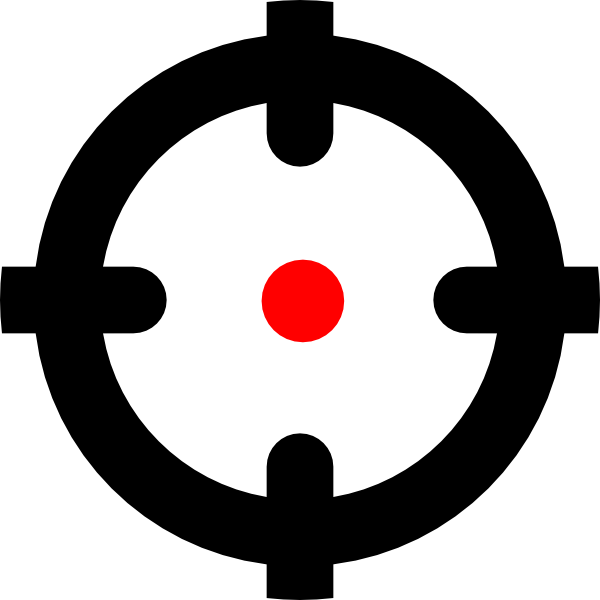
\includegraphics[width=2in, height=2in]{figures/InstalogLogo.png}
\end{center}
\newpage



\tableofcontents
\newpage



\section{Abstract}
The abstract is a brief description of the project which should be
understandable to everyone. Do not use words or acronyms which are not commonly
known. It should state succinctly the objectives, the approach used, suitable
for a person outside the CS domain, summarize what the project is about, what is
achieved, and brief details on its components, issues, etc.
Should be no more than one page.
\newpage



\section{Introduction}
This section is an introduction to the project and will usually be a much longer
version of the Abstract (you can regard this as an expanded version of the
abstract). It should describe the project.
However, unlike the abstract, it should be written for a reader knowledgeable in
computer science. It should also include as numbered subsections:
\begin{itemize}
  \item Relevant background	
  \item Project description (what it is, goals, technical issues, etc.) in more
  technical detail than the abstract; it should include a detailed description of the problem, 
  \item Summary of progress and results obtained,
  \item Related (prior) work, and
  \item Prelude of things to come in the upcoming sections of the report. 
\end{itemize}
You should also describe in this section sources of data (if any), as well as
any topic that you deem to be important.
\newpage



\section{Application}
In this section, you will discuss the application you will build in more detail,
giving the reader a vision about the final product and its capabilities. It
should also point out to
\begin{itemize}
  \item Itemized and prioritized challenges that lie ahead, in terms of the
  algorithms, problems, data integration, etc.
  \item How the project team is planning to address the listed challenges, and
  who in the team is attacking what.
  \item Application Specifications 
\end{itemize}
Algorithms or techniques used to solve these challenges and issues will be
covered in detail in the next section (methodology).
\newpage



\section{Methodology}
This section should discuss any data structure design/maintenance problems, or algorithmic 
problems/challenges, and how they will be/are solved; time and space complexity analysis (if 
needed) of your algorithms, etc. 
\newpage



\section{Software Design}
This section will describe the progress towards the usual software design information, with likely 
components on 
\begin{itemize}
  \item Application Software Requirements
  \item Application Software Specifications
  \item Software Architecture (i.e., client-server architecture; three-tiered
  design, etc.)
  \itemDesign Document
\end{itemize}
\newpage



\section{Project Management and Administrative Details}
Design/update your Gantt chart to show any changes in milestones, timetable, or
responsibility (especially if there are multiple team members). Be sure to
properly indicate who is actually performing each task and the degree of
completion of each task.

Describe how well the project management plan is working. Were there unforeseen
problems with any of the tasks that you have had to work around? Are there
delays in obtaining parts or software? Were major changes to the management plan
or back-up plans required and implemented? What work arounds were necessary to
keep the project on schedule? It is very important that you describe any changes
in the project plan since the proposal and the reasons for them.
Finally, use your management plan to carefully think about what can be
realistically done by your team between now and the end of the semester.
\newpage



\section{User Interface}
This section contains the user interface of the application. It should have
numbered figures with titles and screenshots of the GUI components, as well as
explanations.
\newpage



\section{Testing and Evaluation}
This section should discuss any testing and evaluation done so far.
\newpage



\section{Project Progress}
This section should summarize the progress (or the lack of it) so far, and
address any issues that have arisen recently.
\newpage



\section{Discussion and Conclusions}
These conclusions are not really conclusions since your project is not yet
finished. In this section you should discuss whether the project is on schedule
for completion at the end of the semester. Are there major problems which
require a reevaluation of the project results?  If not, what is the new schedule
and what do you plan to have done by the end of the semester?  You can also
comment on things which have worked better than expected or proved easier to
solve.
\newpage



\section{References}
Any references to the literature, web sites, etc., should follow the ACM
citation standards (Just look at the ACM publications).
\newpage



\section{Appendices}
Use appendices as appropriate. The parts that are necessary are colored in red.
This section can also have, if any, descriptions about background components to
the system and their design:
\begin{itemize}
  \item Database Design.  Simply follow the database design document
  specifications from EECS 341.
  \item User Manual.  This is a manual for users to use the system, describing,
  if any, rules and procedures.
  \item Programmers Manual.  This is a manual for a programmer to take your
  code, install it, use it, understand the code, and revise it if necessary. 
  \item Third-party software use and its incorporation to the project.  Examples
  may be graph drawing software, visualization software, XML-related software, etc. 
  \item Lower-level components such as web services, SOAP functionality,
  AJAX-related design discussions, etc. 
  \item Any figures, drawings, and anything else which is too detailed and/or
  too long to put anywhere else in the report. 
\end{itemize}
\newpage



\end{document}
